\documentclass{poly}
\usepackage{main}

\title{Fonction Inverse}
\author{Terminale STMG2}
\date{}

\begin{document}
\maketitle

\section{Représentation de la fonction inverse}
\begin{definition}
On appelle \textbf{fonction inverse} la fonction définie sur $\left]-\infty;0\right[ \cup \left]0;+\infty \right[$ qui à un nombre $x$ associe le nombre $\dfrac{1}{x}$.
\end{definition}
\begin{remark}
Cette définition indique que la fonction inverse n'est pas définie en $0$. Pour rappel, il est \textbf{interdit de diviser par $0$}.
\end{remark}
\begin{example}
Donner l'inverse de $2; 4; -2; \dfrac{1}{2}; -0,2; 0; 3,25$.
\end{example}
\begin{proposition}
La fonction inverse est représentée par la courbe représentative suivante.
\begin{center}
\includegraphics[width=\textwidth]{Courbe.png}
\end{center}
\end{proposition}
\newpage
\section{Dérivée de la fonction inverse}
\begin{proposition}
La fonction inverse est dérivable sur $\left]-\infty;0\right[ \cup \left]0;+\infty \right[$, et sa dérivée est définie par
\begin{equation*}
x \mapsto - \dfrac{1}{x^2}
\end{equation*}
\end{proposition}
\begin{proposition}
La fonction inverse est \textbf{décroissante} sur $\left]-\infty;0\right[$, et \textbf{décroissante} sur $\left]0;+\infty \right[$.
\end{proposition}
\begin{center}
\begin{tikzpicture}
\tkzTabInit{$x$/1, Signe de $f'(x)$/1, Variations de $f$/2}{$-\infty$, $0$, $+\infty$};
\tkzTabLine{,-,d,-,};
\tkzTabVar{+ /, -D+ / /, - /};
\end{tikzpicture}
\end{center}
\begin{remark}
La fonction inverse n'est pas décroissante sur son ensemble de définition (c'est-à-dire $]-\infty;0[\cup]0;+\infty[$). Par exemple $\dfrac{1}{-2} < \dfrac{1}{2}$, alors que $-2 < 2$. Cela souligne l'importance de la valeur interdite $0$.
\end{remark}

\newpage

\section{Comportement assymptotique}

\begin{tcolorbox}
\begin{remark}
On appelle $f$ la fonction inverse définie sur $\R^*$. Alors,
\begin{itemize}
\item Plus les valeurs de $x$ augmentent, et plus la valeur de $f(x)$ diminue et se rapproche de $0$.
\item Plus les valeurs de $x$ se rapprochent de $0$ \textbf{en restant positives}, et plus la valeur de $f(x)$ est grande. 
\end{itemize}
On constate un comportement similaire quand on observe le comportement de $f(x)$ pour des valeurs de $x$ négatives.       
\end{remark}
\end{tcolorbox}


\begin{proposition}
Soit $f$ la fonction inverse. Alors,

\begin{minipage}{0.2\textwidth}
\begin{equation*}
\lim_{x \to -\infty} \dfrac{1}{x} = 0
\end{equation*}
\end{minipage}
\hfill
\begin{minipage}{0.2\textwidth}
\begin{equation*}
\lim_{x \to 0^-} \dfrac{1}{x} = -\infty
\end{equation*}
\end{minipage}
\hfill
\begin{minipage}{0.2\textwidth}
\begin{equation*}
\lim_{x \to 0^+} \dfrac{1}{x} = +\infty
\end{equation*}
\end{minipage}
\hfill
\begin{minipage}{0.2\textwidth}
\begin{equation*}
\lim_{x \to +\infty} \dfrac{1}{x} = 0
\end{equation*}
\end{minipage}
\end{proposition}
\begin{center}
\includegraphics[width=\textwidth]{Assymptotes.png}
\end{center}
\begin{definition}
On dit que la courbe représentative de la fonction inverse :
\begin{itemize}
\item admet une assymptote horizontale d'équation $y = 0$ en $-\infty$ et en $+\infty$;
\item admet une assymptote verticale d'équation $x = 0$. 
\end{itemize}
\end{definition}

\begin{remark}
Le tableau de variation de la fonction inverse peut être complété ainsi.
\end{remark}
\begin{center}
\begin{tikzpicture}
\tkzTabInit{$x$/1, Variations de $f$/2}{$-\infty$, $0$, $+\infty$};
\tkzTabVar{+ / $0$, -D+ /$-\infty$ / $+\infty$, - / $0$};
\end{tikzpicture}
\end{center}
\end{document}